\chapter{Introduzione}

\section{Cos'\`e lo Spider Keyer?}
\begin{center}
	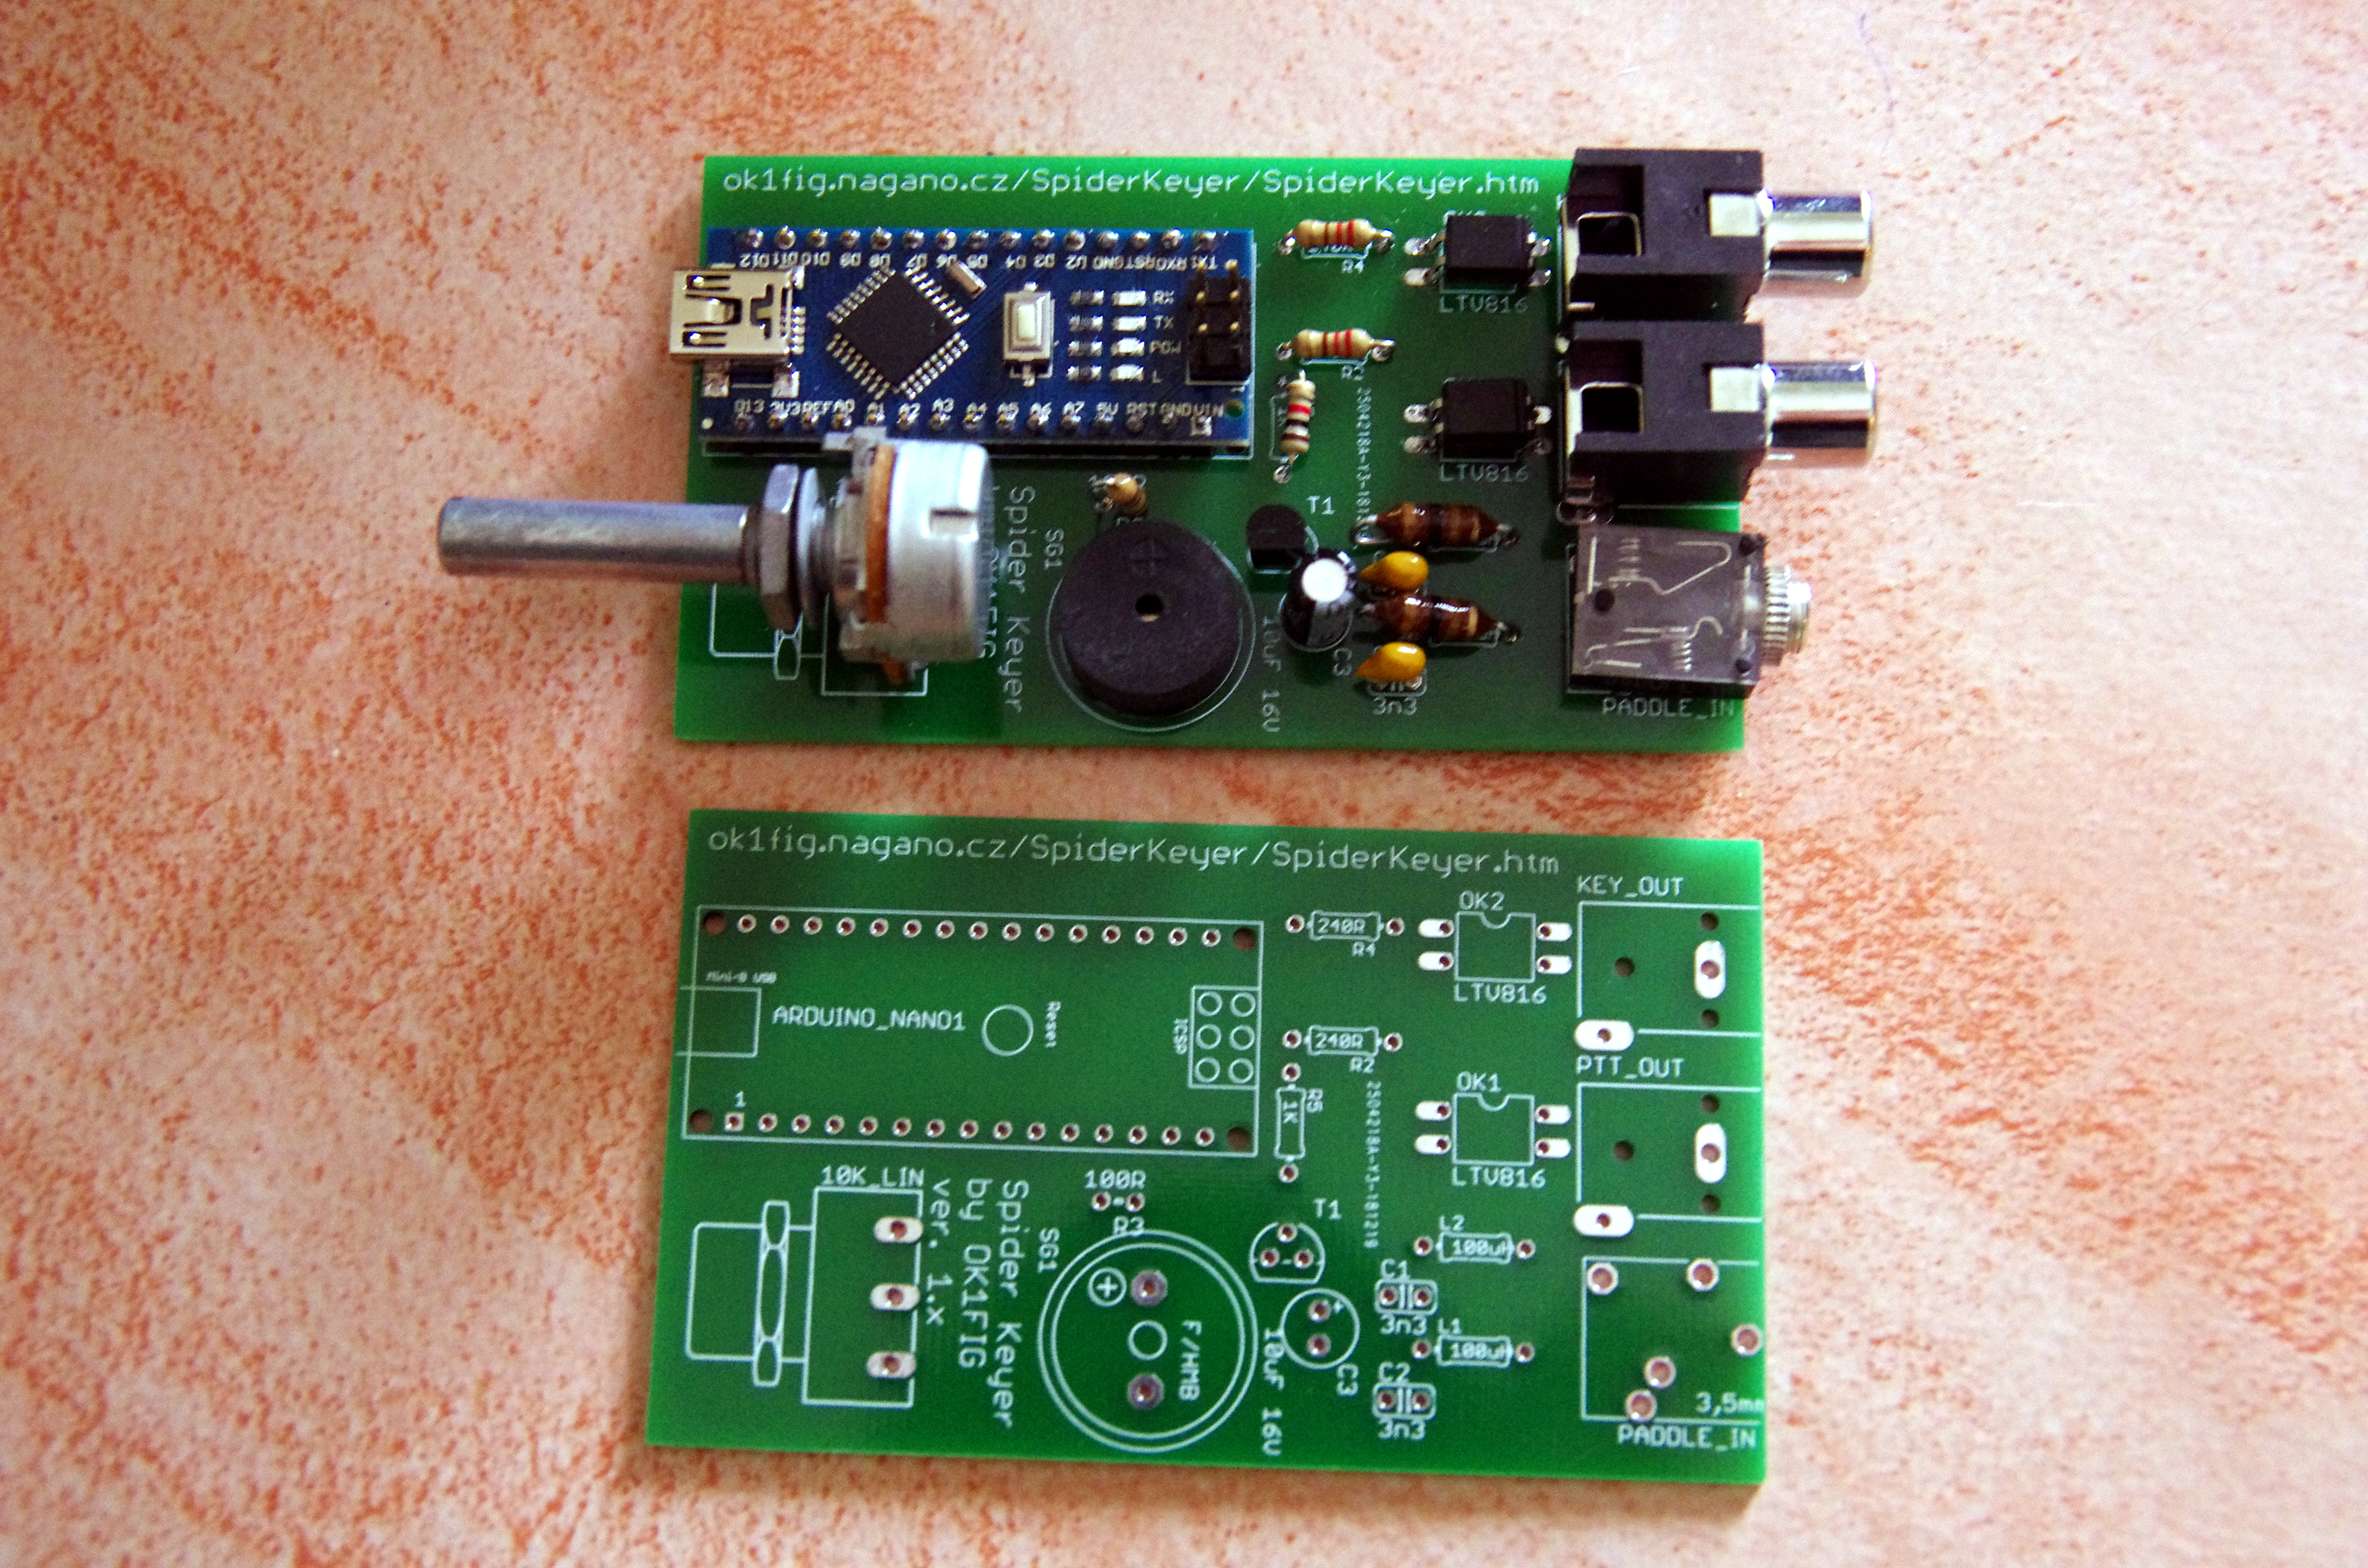
\includegraphics[width=\linewidth]{./IMGP4418.JPG}
\end{center}
Lo Spider Keyer \`e un keyer per tasti telegrafici elettronici progettato da Petr Mal\'y (OK1FIG) per essere estremamente compatto (la parola "Spider" sta a indicare che pu\`o essere lasciato penzolare tra i cavi dietro la stazione radio) e per poter comunicare sia con la radio (fungendo da generatore di dit e dah per le radio che supportano solo il tasto meccanico) che con il PC (in particolar modo connettendosi al software Ham Racer, scritto dallo stesso OK1FIG).
Connettendo sia PC che radio \`e possibile generare automaticamente i dit e dah a partire da un testo digitato.

Questo manuale \`e stato scritto integrando le informazioni fornite dall'autore alla pagina \url{http://ok1fig.nagano.cz/SpiderKeyer/SpiderKeyer.htm} con la mia esperienza personale di costruzione e utilizzo.

\section{Caratteristiche}
L'interfaccia hardware \`e estremamente semplice per ridurre al minimo le dimensioni (utilizzando i file Gerber inclusi, lo Spider Keyer misura $4.9 \times 8.3$ cm). Sono presenti infatti:
\begin{itemize}
	\item un connettore jack da 3.5mm per il tasto elettronico;
	\item due connettori RCA per l'uscita verso la radio (uno per il segnale, l'altro per controllare il PTT);
	\item una porta mini USB per l'alimentazione e per la comunicazione con il PC;
	\item un potenziometro per la regolazione della velocit\`a.
\end{itemize}

Viceversa l'interfaccia software \`e molto completa e consente una regolazione fine di svariati parametri tramite comunicazione seriale (vedi sezione \ref{sec:cmds}).